
\chapter{Functional analysis}
\label{chapter:functional analysis}

\section{Infinite dimensions}


\recommended{A very pedagogical text. Covers metric spaces, Banach spaces, Hilbert spaces, the fundamental theorems like the Hahn--Banach theorem, open mapping theorem, closed graph theorem. Spectral theory of self-adjoint operators, applications to quantum mechanics. (This makes the book special, together with its pedagogical level.)}{images/Kreyszig_frontpage}

\recommended{A classic in PDE theory. Used in many graduate courses all over the world.}{images/Evans-frontpage}

\recommended{A classic. Maybe not the most accessible text, but it is very much geared towards mathematical physics.}{images/Reed_Simon_frontpage}

\recommended{Eberhard Zeidler was a giant of nonlinear functional analysis, and enormously productive. Many of his volumes focus greatly on pedagogical exposition and motivation for study. This book is no exception.}{images/Zeidler-frontpage} 

We now enter the realm of inifinite dimensional vector spaces. The mathematical field that studies such objects is called \emph{Functional Analysis}. Infinite dimensional vector spaces are often spaces of \emph{functions}. We know that operators like the derivative acts linearly on differentiable functions. Hence, \emph{functional analysis is the mathematical language of analysis of partial differential equations}.

In quantum chemistry, our laws of nature are \emph{linear}, e.g., the time-independent Schr\"odinger equation is a \emph{linear partial differential equation}. On the other hand, many of our approximation methods are \emph{nonlinear} in nature. Such methods comprise self-consistent field methods like Hartree--Fock and density-functional theory, complete-active space self-consistent field theory, and coupled-cluster theory. Hartrr--Fock, for example, can be viewed as a coupled set of nonlinear integro-partial differential equations. The mathematical analysis of these methods then needs \emph{nonlinear functional analysis}. Since most methods are formulated in terms of optimization of some energy function, we must deal with \emph{nonlinear optimization} in infinite dimensions. There are also methods, like many-body perturbation theory, that are not variational, but instead needs the abstract theory of \emph{perturbation theory} in order to be studied.

All these topics are fairly advanced, and usually encountered only after a few semesters' mathematics studies. The published mathematics papers that study quantum chemical methods mathematically are brilliant and truly inspiring works of famous mathematicians such as P.-L.~Lions, E.H.~Lieb, B.~Simon, and T.~Kato, to name a few. Hence, this section will only mention some concepts and try to draw some lines, to get a feel for the concepts that the mathematician works with. Maybe it can be a help to read and understand mathematics papers on quantum chemistry methods, and to bridge a language barrier that certainly is present.




\subsection{Introducing infinite dimensions}

We have previously studied finite-dimensional vector spaces. However, quantum mechanics is formulated with an infinite dimensional vector space -- a separable Hilbert space. The quantum chemist may say, ``but we always introduce a basis set, and then we are in finite dimensions!'' True, but the underlying physical model can \emph{not} be formulated in finite dimensions. For example, if we consider quantum mechanics in one spatial dimension, the canonical commutator relation
\begin{equation}
    [\hat{x}, \hat{p}_x] = \rmi \hbar \mathbbm{1}
\end{equation}
requires infinite dimensions. Furthermore, in order to prove error estimates of some quantum chemical model, one needs to in some way compare the finite dimensional model with the infinite dimensional ``exact'' model. This is best done by basically working in the infinite dimensional setting all the time, considering instead finite dimensional subspaces of the function spaces involved. [Quantum chemists are used to talking about the full-configuration interaction limit as ``exact''. It is not! One still has the basis set error. This can not be eliminated in finite dimensions.]

In Definition~\ref{def:vector-space}, Section~\ref{sec:general-finite-dimensional}, we introduced a general vector space. There is no reason why a general vector space should have a finite dimension. Here are some examples of vector spaces that have infinite dimension:

\begin{myExample}{Space of all functions over a set}{}
    Let $S$ be a set. The space of all functions $f : S \to \FF$ is a vector space, with addition and scalar multiplication defined pointwise,
    \begin{equation}
        [f + g](x) = f(x) + g(x), \quad [\alpha f](x) = \alpha f(x).
    \end{equation}
    The dimension of this space is at least as large as the cardinality of $S$. To see this, let $y \in S$ be arbitrary, and let $f_y : S \to \FF$ be the function defined by $f_y(x) = 0$ if $x\neq y$ and $f_y(y)=1$. These functions are linearly independent. Thus every point in $S$ gives a linearly independent vector.
    
    Special cases: $S = \NN$ gives the set of all sequences. $S = \{1,2,\cdots,N\}$ gives $\FF^n$ (without the inner product, which is extra information).
\end{myExample}

\begin{myExample}{Space of all polynomials}{}
    The space of all polynomials $p : \FF\to\FF$ with coefficients in $\FF$ is a vector space. If we set $S = \FF$ in the previous example, the space of all polynomials is a subspace of the space of all functions from $\FF$ to $\FF$. An arbitrary element of our vector space can be written as
    \[ p(x) = a_0 + a_1 x + a_2 x^2 + \cdots a_n x^n \]
    for a vector $\mathbf{a} = [a_0, \cdots, a_n] \in \FF^{n+1}$. Note that $n$ depends on $p$, and is not bounded, so the dimension is infinite. In particular the monomials $x^n$ are linearly independent, and there are infinitely many of these. 
\end{myExample}

\begin{myExample}{Space of continuous functions}{}
Let $\Omega \subset \RR^n$ be a bounded, closed domain, such as a box $[0,1]^n$ which includes its boundary. Consider  the set $C^k(\Omega)$ of functions that are continuous at all points in $\Omega$, with continuous partial derivatives of order $\leq k$. (See Chapter~\ref{sec:differentiability}.) Consider in particular the special case $k=0$. We can supply a norm on this space,
\begin{equation}
\|f\|_\infty = \max \left\{ |f(x)| \mid x \in \Omega \right\}.
\end{equation}
The maximum can be shown to be attained, since $\Omega$ is bounded and closed, and hence compact. (We have not covered compactness so far in the lecture notes.) It is a fact that $C^0$ is complete with this norm. This means. that if $f_k \in C^0(\Omega)$ is a sequence of continuous functions, and if
\begin{equation}
    \|f_j - f_k\|_\infty =\max\{ |f_j(x)-f_k(x)| \mid x \in \Omega \}
\end{equation}
is a Cauchy sequence, then it converges to some $f\in C^0(\Omega)$, a continuous function. The completeness can be generalized to $C^k$, but we have to modify the norm accordingly.
\end{myExample}
\todo{Add plots illustrating the norm and convergence.}

\begin{myExample}{$N$-electron Hilbert space}{}
    This is the main vector space of quantum chemistry, and a central ingredient in the mathematical formulation of molecular problems in the Born--Oppenheimer approximation. This space is constructed as follows: Let $X = \RR^3 \times \{\uparrow, \downarrow\}$ be two copies of Euclidean space. Here, $\uparrow$ and $\downarrow$ are simply symbols that we associate with spin up and down (``$\alpha$'' and ``$\beta$'' spin). The set $X$ is made into a measure space by assigning the product of Lebesgue measure and counting measure (see Chapter~\ref{sec:measure-and-integration}). We now can define \emph{single-electron space} $\mathcal{H}_1 = L^2(X;\CC)$. For multiple electrons, we take \emph{the antisymmetric tensor product $N$ times},
    \begin{equation}
        \mathcal{H}_N = \mathcal{H}_1 \wedge \mathcal{H}_1 \cdots \wedge \mathcal{H}_1 \quad \text{($N$ times)}.
    \end{equation}
    The elements of $\mathcal{H}_N$ now become antisymmetric upon permutation of the particle indices, i.e., for all pairs $(i,j)$, 
    \[ \psi(x_1,\cdots, x_j, \cdots, x_i, \cdot ,x_N) = - \psi(x_1, \cdots, x_i, \cdots, x_j, \cdots, x_N). \]
    
    By theorems on spaces of square integrable functions, we have the alternative characterization: $\psi \in \mathcal{H}_N$ if and only of $\psi \in L^2(X^N)$ and is antisymmetric. Since $X^N$ can be viewed as $2^N$ copies of $\RR^{3N}$ associated with the $2^N$ unique arrangements of $N$ spins, we also have $\psi \in L^2(\RR^{3N})^N$, i.e., $\psi$ is a \emph{vector of functions}. These functions are \emph{not necessarily} antisymmetric, since they isolate the spatial coordinate.
\end{myExample}

The infinite dimensional spaces we meet in functional analysis are often \emph{spaces of functions}. These spaces, when supplied with a suitable topological structure, are designed to deal with partial differential equations. Here is an example that shows how this is done for a simple PDE:

\begin{myExample}{Poisson equation}{}
(For this example, we use nomenclature from Chapter~\ref{sec:calculus}.)
Let $\Omega = ]0,1[^3 \subset\RR^3$ be an open box, a typical domain with a well-behaved boundary $\partial\Omega$.
Consider the Poissin equation, a PDE, formulated ``classically'': Find $u : \Omega \to \RR$ such that
\begin{align}
 \nabla^2 u(\bvec{x}) &= f(\bvec{x}), 
  \quad \bvec{x} \in \Omega \\
 u(\bvec{x}) &= 0, \quad \bvec{x}\in\partial\Omega
\end{align}
where $f : \RR^3\to \RR$ is some function,
and such that $u(\bvec{x}) = 0$ on $\partial\Omega$. What is meant by a solution to this equation? Should we require $u$ to have continuous derivatives up to and including second order? Is it enough that the second order derivatives exist? What are the properties of the ``data'' $f$? These questions must be answered, such that one can provide a sound theory for existence and uniqueness of solutions.

If we introduce the Sobolev space $H^1_0(\Omega)$ of twice weakly differentiable functions over $\Omega$ that vanishes on the boundary, this is a Hilbert space. In fact the Laplace operator $\nabla^2$ is a continuous operator from $H^1_0(\Omega)$ into the space $H^{-1}_0(\Omega)$, which is a set that also contains some generalized functions, i.e., functions that are not really functions, but make sense when we integrate them. It is big! Then, the PDE can be formulated as: Given $f \in H^{-1}_0(\Omega)$, find $u \in H^1_0(\Omega)$ such that 
\begin{equation}
 \hat{A} u = f. 
\end{equation}
Now, one can show that $\nabla^2 = \hat{A} : H^1_0\to H^{-1}_0$ is in fact not only continuous, but also invertible, with a continuous inverse. Then, there exists a unique solution $u = \hat{A}^{-1} f$ that depends \emph{continuously} on $f$. 

Now, one can introduce the \emph{Galerkin method}: Choose a finite dimensional subspace $V \subset H^1_0(\Omega)$ with basis $\{b_i\}$. For example, a finite element space. This space is suitable for approximation, in the sense that we can refine the finite element mesh and obtain approximations of any accuracy of elements in $H^1_0$. The PDE becomes a linear algebra problem,
\begin{equation}
    A \mathbf{u} = \mathbf{f},
\end{equation}
with $A_{ij} = \braket{b_i,\hat{A} b_j} = \braket{\nabla b_i,\nabla b_j}_{L^2}$ and $f_j = \braket{b_k, f}_{L^2}$.

From the structure of the function spaces and the Galerkin space, we know that this approximation is convergent as the mesh becomes finer. We even have error estimates.

This methodology is quite powerful, and amply motivates the study of functional analysis for studying PDEs.
\end{myExample}
\todo{Elevate this example to a section.}

\subsection{Banach spaces and Hilbert spaces}

In Section~\ref{sec:topological-vector-spaces}, we introduced the inner product spaces and normed spaces. However, the spaces that are most useful in analysis are \emph{complete spaces}: Accroding to Definition~\ref{def:cauchy-complete} a space is complete if all sequences that ``ought to converge'' actually converges. All possible limits of sequences are present, and there are no holes, so to speak, in the space.

\begin{myDefinition}{Banach and Hilbert space}{banach-hilbert}
    A \emph{Banach space} is a complete normed vector space. A \emph{Hilbert space} is a complete inner product space.
\end{myDefinition}
All Hilbert spaces are Banach spaces, but not vice versa.


Infinite dimensional spaces can be \emph{huge}. Usually, we will be mostly interested in separable spaces:
\begin{myDefinition}{Separable space}{separable}
A Banach space $X$ is called \emph{separable} if it contains a dense countable subset, i.e., a countable $A \subset X$ such that the closure of $A$ is $X$. 
\end{myDefinition}


Recall that a subset $A\subset V$ is dense if its closure is $V$. For example, the rationals $\QQ$ are dense in $\RR$. A space is separable if there exists some \emph{list of elements} that form a dense subset: all elements of the space can be written as limits of sequences of elements taken from this list. This seems rather drastic, but thankfully, most spaces of interest to us are separable.


\section{$L^p$ spaces (Lebesgue spaces)}


Consider some open subset $\Omega \subset \RR^n$, with a ``nice'' boundary (e.g., piecewise smooth) and consider the set of measurable functions $f : \Omega \to \FF$. (See Section~\ref{sec:measure-and-integration} on measure and integration theory. Measurable functions are roughly those that have an integral, even if it may be infinite.) We have previously encountered the $L^p$-spaces.

Recall the fact that $[f]\in L^p(\Omega)$ is an equivalence class of almost-everywhere equal functions. We now have the strange situation that \emph{this is almost universally ignored}; one writes things like ``Let $f$ be defined as [some definition] be a function, and we now show that $f \in L^p$''. Only when there is doubt about some property, e.g., a singularity, one suddenly reintroduce the notion of equivalence class. Talk about abuse of notation! So this is something to be aware of.

We also have the case $p = +\infty$, but then the norm is not defined as an integral, but rather the \emph{essential supremum}:
\begin{equation}
    \|f \|_\infty := \operatornamewithlimits{ess sup}_{x\in\Omega} |f(x)|,
\end{equation}
where the \emph{essential supremum} means 
\begin{equation}
    \operatornamewithlimits{ess sup}_{x\in\Omega} |f(x)| := \inf \{ \sup_{x \in \Omega\setminus Z} |f(x)| \mid Z \text{ has zero measure} \}.
\end{equation}
This is a bit of a mouthful, but it essentially means ``maximum, but try to take away point sets of zero measure to lower the value''. The space $L^\infty$ is not separable.

\begin{myDefinition}{Almost everywhere}{ae}
Let $f$ be a measurable function over a measure space. Let $P(f(x))$ be a statement, such as ``$|f(x)|<1$. We say that $P(f(x))$ holds \emph{almost everywhere} if it holds everywhere except for a set of measure zero.
\end{myDefinition}

\begin{myExample}{Coulomb potential}{}
In the analysis of the molecular Schrödinger equation, we must deal with the singular Coulomb potential between charged particles. For the hydrogen atom in the Born--Oppenheimer approximation,
\begin{equation}
V(\bvec{r}) = \frac{1}{r} = \frac{1}{\|\bvec{r}\|} = \frac{1}{\sqrt{x^2 + y^2 + z^2}}.
\end{equation}
As a function $1/r$ does not live in any of the $L^p$ spaces due to the singularity at the origin. On the other hand, the physics of the Coulomb potential has a short-range and a long-range part. The short-range part is responsible for the \emph{nuclear cusp} in the wavefunction, while the long-range part is responsible for the infinite scattering cross section. Thus, we split $V$ into a long-range and a short-range part, by introducing some ball $\Omega = B_R(\RR^3)$ and setting
\begin{equation}
V = V_\text{sr} + V_\text{lr} = \frac{1}{r} \chi_\Omega + \frac{1}{r}\chi_{\Omega^\complement}.
\end{equation}
Now the long range part is clearly bounded by $1/R$,
\begin{equation}
    V_\text{lr} \in L^\infty(\RR^3),
\end{equation}
while the short-range part can be shown to be
\begin{equation}
    V_\text{sr} \in L^p(\RR^3), \quad p \in [1,2].
\end{equation}
For analysis, the value $p=3/2$ is often taken, giving
\begin{equation}
    V \in L^{3/2}(\RR^3) + L^\infty(\RR^3),
\end{equation}
where the right-hand side is defined as the space of functions splittable as a sum with terms from each space. (This is in fact a Banach space when the proper norm is supplied.)

Thus, we see how Banach spaces can be used to handle some  singular potentials. This can in turn help with formulating the Schr\"odinger equation in a rigorous manner.
\end{myExample}

\subsection{The weak derivative}

Studying PDE, one needs partial derivatives of functions in $L^p$-spaces. However, we have seen that such functions are only defined up to a set of measure zero. In order to define partial derivatives of $L^p$ functions, we need a strategy that deals with this. The solution is the \emph{weak derivative}.

We first need the notion of a test function.
\begin{myDefinition}{Test functions}{}
    Let $\Omega\subset\RR^n$ be open.
    A \emph{test function} is an infinitely differentiable function $f : \Omega \to \FF$ with compact support, i.e., there is some closed and bounded set $K \subset \Omega$ such that $f$ is identically zero on $K^\complement$.

    The set of test functions is denoted $C^\infty_0(\Omega)$.
\end{myDefinition}
Test functions exist. The classic example is the following:
\begin{myExample}{The bump function}{bump}
    Let $u : \RR^n \to \RR$ be given by
    \begin{equation}
        u(\bvec{x}) = \begin{cases} 0 & \|\bvec{x}\| \geq 1 \\
        \exp(-1/(1 - \|\bvec{x}\|^2)) & \|\bvec{x}\| < 1
        \end{cases}
    \end{equation}
    Then $u$ is infinitely many times differentiable, in particular across the boundary of the unit sphere, too. See Fig.~\ref{fig:bump}.
\end{myExample}
\begin{figure}
    \centering
    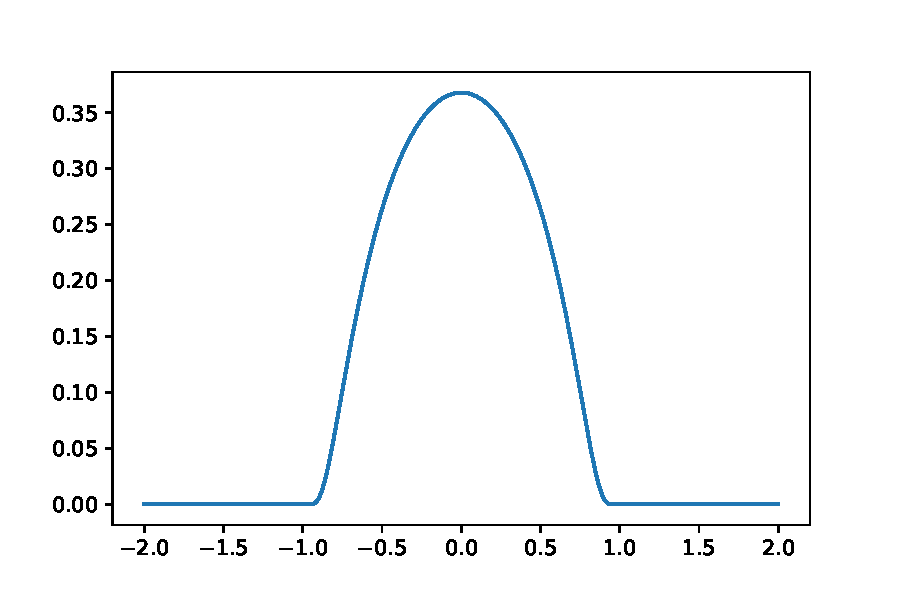
\includegraphics{illustrations/bump.pdf}
    \caption{The bump function from Example~\ref{ex:bump} in one dimension.}
    \label{fig:bump}
\end{figure}
From the above example, a huge number of test functions can be generated by \emph{convolution}: Let $\eta = u/\int u$, normalizing the bump. Take any integrable function $f : \RR^n\to\CC$, and take the convolution with $\eta$,
\begin{equation}
    f_\epsilon(\bvec{x}) = \int_{B_1(0)} \epsilon^{-n} \eta(\bvec{y}/\epsilon) f(\bvec{x}-\bvec{y}) \, \rmd\bvec{y}.
\end{equation}
This process smooths $f$, and is called \emph{mollification of $f$}. For small $\epsilon$, the function is only ``slightly'' modified, since the bump becomes very concentrated. In particular, if $f$ is supported in $K$, then $f_\epsilon$ is supported in only a slightly larger $K_\epsilon$.

In fact the set of test functions is \emph{dense} in all the $L^p$ spaces except $L^\infty$. [Check precise wording of this.] All $L^p$ functions can be arbitrarily well approximated by such functions. Can you guess a construction of the approximate sequence for a given $f \in L^p(\Omega)$?

\todo{Produce a visualization.}

Having established the set of test functions, we can now define the weak derivative:
\begin{myDefinition}{Weak derivative/distributional derivative}{weak-derivative}
Let $f \in L^1_\text{loc}(\Omega)$ be a \emph{locally integrable function}. This means that $f \in L^1_\text{loc}(K)$ for all bounded subsets $K \subset \Omega$. (This function set is very general, and contains all the $L^p$ spaces!)

A measurable function $g_k$ is called \emph{a weak derivative} of $f$ if, for all test functions $\varphi\in C^\infty_0(\Omega)$,
\begin{equation}
    \int \varphi(\bvec{x}) g_k(\bvec{x}) \; \rmd \bvec{c} = - \int \pdiff{\varphi(\bvec{x})}{x_k} f(\bvec{x}) \; \rmd \bvec{x}.
\end{equation}
We see that the weak derivative behaves just like the derivative of $f$ when being under the integral sign and ``tested against'' a test function.

Weak derivatives of higher order are defined completely analogously. 
Let $\alpha = (\alpha_1,\cdots,\alpha_k)$ denote a multi-index of nonnegative integers, and define 
\begin{equation}
    \partial^\alpha = \pdiff{^{\alpha_1}}{x_1^{\alpha_1}}\pdiff{^{\alpha_2}}{x_2^{\alpha_2}}\cdots\pdiff{^{\alpha_n}}{\alpha_n^{\alpha_n}}, \quad |\alpha| = \sum_{i=1}^n \alpha_i
\end{equation}
$g_\alpha \in L^1_\text{loc}$ is a weak partial derivative of mixed order $\alpha$ if
\begin{equation}
    \int \varphi(\bvec{x}) g_\alpha(\bvec{x}) \; \rmd \bvec{x} = (-1)^{|\alpha|} \int \partial^\alpha{\varphi(\bvec{x})} f(\bvec{x}) \; \rmd \bvec{x}.
\end{equation}
Mixed weak derivatives are symmetric. The weak derivative is unique up to a set of measure zero.

\end{myDefinition}

\subsection{Sobolev spaces}

A very important class of function spaces are Sobolev spaces.
\begin{myDefinition}{Sobolev space}{sobolev}
    Let $\Omega \subset \RR^n$ be open. Let $p \in [1,+\infty]$ (incliuding infinite).
    Let $u \in L^p(\Omega)$, and suppose $u$ has weak derivatives up to order $k \geq 1$ that are \emph{also} in $L^p(\Omega)$. Then we say that $u \in W^{k,p}(\Omega)$, a Sobolev space. The Sobolev space $W^{k,p}(\Omega)$ is a Banach space with norm
    \begin{equation}
    \|u\|_{W^{k,p}} = \|u\|_p + \sum_{\alpha, |\alpha|\leq k} \|\partial_\alpha u\|_p,
    \end{equation}
    where $\alpha$ denotes a partial derivative of order $\leq k$. [For example, order 1 means $\alpha\in\{1,\cdots,n\}$, order 2 means $\alpha = (\alpha_1,\alpha_2)$ with $\alpha_i \in \{1,\cdots,n\}$, and so on.]
\end{myDefinition}

For encoding \emph{boundary conditions}, it is useful to consider Sobolev spaces of functions that in some ``integrable sense'' vanish on $\partial \Omega$.
\begin{myDefinition}{Sobolev space, homogenous boundary conditions}{}
Let $\Omega\subset \RR^n$ with piecewise smooth boundary. The space $W^{k,p}_0(\Omega)$ is defined as the clousure in the $W^{k,p}(\Omega)$ norm of the set of test functions $C^\infty_0(\Omega)$.
\end{myDefinition}
The definition may seem arbitrary, but the denseness of the test functions in $W^{k,p}(\RR^n)$ implies that this makes sense, and indeed corresponds to functions that vanish near the boundary, when $k>0$. When $k=0$ we just get $L^p(\Omega)$.

\section{Hilbert spaces}

\subsection{$L^2$ -- the square integrable functions}

For a quantum chemist, the most important $L^p$ space is $L^2(\Omega)$, where $\Omega$ is a measure space, such as $\RR^3$, or $X = \RR^3 \times \{\uparrow,\downarrow\}$. Previously, we saw that this was a Banach space with the $L^2$ norm, but this norm comes from an inner product:
\begin{equation}
    \braket{f,g}_{L^2} := \int_\Omega \overline{f(x)} g(x) \, \rmd x,
\end{equation}
where the complex conjugate is relevant only if $\FF = \CC$. Again, functions that agree on sets of measure zero are identified.

\subsection{$\ell_2$ -- the archetypal separable Hilbert space}

Consider the following situation: Let $u = (u_i) \subset \FF$ be a real or complex-valued sequence. Let $p \in [1,+\infty)$. We can define a norm given by
\begin{equation}
    \|u\|_p := \left(\sum_{i\in\NN} |u_i|^p \right)^{1/p}.
\end{equation}
The set of sequences such that $\|u_p\|$ is a convergent sum is called $\ell_p$. For $p=+\infty$, we set $\|u\|_{+\infty} = \max_i |u_i|$. The spaces $\ell_p$ are all Banach spaces.

In particular, the space $\ell_2$ is a Hilbert space when we use the inner product
\begin{equation}
    \braket{u,v} = \sum_{i\in\NN} \overline{u_i} v_i.
\end{equation}
This Hilbert space is an archetypal Hilbert space, as we will next see.

\subsection{Existence of orthonormal bases}

\todo{This section needs more work.}

The following fact is significant, because it tells us that $\ell_2(\NN;\FF)$ is an archetypal separable Hilbert space, much in the same manner as $\FF^n$ is the archetypal finite-dimensional Hilbert space.


\begin{myDefinition}{Orthnormal basis for separable Hilbert space}{}
An orthonormal basis for an infinite dimensional separable Hilbert space $V$ is a linearly independent orthonormal set $\{b_i\}\subset V$ (i.e., $\braket{b_i,b_j} = 0$ whenever $i\neq j$, and $\braket{b_i,b_i} = 1$), such that for every $u \in V$, there exist numbers $c_i \in \FF$ such that
\begin{equation}
    u = \sum_{i=1}^\infty c_i b_i.
\end{equation}
The infinite sum is to be interpreted as a \emph{series}, i.e., $u \in V$ means
\begin{equation}
    \|u - \sum_{i=1}^N c_i b_i\| \to 0 \quad \text{as} \quad N\to+\infty.
\end{equation}

The space of sequences equipped with the Euclidean inner product is denoted $\ell_2(\NN)$,
\begin{equation}
    \braket{c,d}_{\ell_2} = \sum_{i=1}^\infty \overline{c_i} d_i.
\end{equation}
We see that $V$ and $\ell_2$ are \emph{isometrically isomorphic} when a basis is given, since if $v = \sum_i d_i b_i$ then $\braket{u,v}= \braket{c,d}_{\ell_2}$.
\end{myDefinition}

An fundamental result is the following:
\begin{myTheorem}{}{}
Any separable Hilbert space has an orthonormal basis.
\end{myTheorem}
Thus any separable Hilbert space is essentially $\ell_2(\NN)$ after a basis has been chosen.  





% \subsection{More general domains}


% In the definition of the $L^p$ spaces, we used a domain $\Omega \subset \RR^n$ for our definition. But the important thing is that $\Omega$ is a \emph{measure space}. This notion generalizes computing volumes in space, and an important instance is the Cartesian product $\Omega \times D$, where $D$ is a discrete set, such as $D = \{\uparrow,\downarrow\}$ for the two values of electron spin. Thus, $\Omega \times D$ becomes two copies of $\Omega$, one with spin up and one with spin down. Equipping $D$ with \emph{counting measure} (mathematicians are good at making counting abstract!) we obtain for the integral (denoting $\xi = (x,j) \in \Omega\times D$),
% \begin{equation}
%     \int_{\Omega\times D} f(\xi) \, \rmd \xi := \sum_{j \in D} \int_\Omega f(x,j) \, \rmd x.
% \end{equation}
% Sometimes, one thinks of $f$ as two separate ``component'' functions $f_j(x)$, and this is ok. Case in point: spin up and spin down components of a single-electron wavefunction.

\section{Linear transformations}

We now scratch the surface on linear transformations on infinite dimensional Banach and Hilbert spaces.
    
Let $V$ be a separable Hilbert space. We now know that we may think of this space as the coneptually simpler space $\ell_2 = \ell_2(\NN)$, the space of square summable sequences. In particular, there is no notion of having to consider equivalence classes of functions defined almost everywhere.

In the finite dimensional case, linear transformations between vector spaces became matrices. How about in the separable Hilbert space case? Do linear transformations and operators become infinite matrices?

Yes and no. One can certainly define a class of linear transformations using infinite matrices, if one is careful. However, the set of linear transformations on a Hilbert space is much richer than the corresponding finite dimensional linear transformations. For a given basis choice a linear transformation may or may not have a well-defined matrix representation.


Perhaps the most important fact is that \emph{transformations need not be continuous}. In the finite-dimensional case, all linear transformations were continuous, even though we did not discuss this fact: In finite dimensions, there is no way for a linear transformation to produce rips or tears or jumps. Moreover, even if linear transformations is continuous, there are some  that are ``more continuous'' than others, such as compact operators, Hilbert--Schmidt operators, trace-class operators, and merely continuous operators.

Since the topology on a Banach or Hilbert space is translationally invariant, a linear transformation $T: V \to W$ between two Banach spaces is continuous at $x \in V$ if and only if it is continuous at $0$, and then continuity is equivalent to \emph{boundedness}, i.e., a finite operator norm:
\begin{myDefinition}{Bounded linear transformations}{bounded transformations}
    Let $V$ and $W$ be Banach spaces over $\FF$, and let $D(T) \subset V$ be a linear subspace.Let $T : V \to W$ be a linear transformation, i.e., for all $u,v \in D(T)$ and all $\alpha \in \FF$,
    $$ T(\alpha u) = \alpha Tu, $$
    and
    $$ T(u + v) = Tu + Tv. $$
    The linear space $D(T)$ is called the \emph{domain of $T$}, and it may or may not be all of $T$.
    Let $\|T\|_{L(V,W)}$ be the norm (``operator norm'') defined by
    \begin{equation}
        \|T\|_{L(V,W)} = \sup \left\{ \frac{\|T u\|_W}{\|u\|_V} \mid 0 \neq u \in D(T) \right\}.
    \end{equation}
    If $\|T\|_{L(V,W)}< +\infty$ and $D(T) = V$, then $T$ is a \emph{bounded, or countinuous, linear transformation from $V$ to $W$}.
\end{myDefinition}
In the definition, note that we introduce the domain $D(T)$ of $T : V \to W$. The reason is that operators that are not bounded usually cannot be defined on all of $V$. On the other hand, if $T$ is bounded on $D(T)$ the \emph{bounded linear transformation theorem} states that $T$ can be unuqiely \emph{extended} to all of $V$. This is why we eliminate the domain in the definition of the space $L(V,W)$ of bounded linear transformations.

\begin{myTheorem}{Bounded linear transformations are continuous}{}
    Any $T \in L(V,W)$ is a continuous function.    
\end{myTheorem}


We now give an examples of linear transformations that are \emph{unbounded}, i.e., not bounded.

\begin{myExample}{Unbounded operator}{}
    Let $\ell_2(\NN,\RR)$ be the space of square summable sequences of real numbers, i.e., $u = (u_n) \subset \RR$ with 
    \[ \sum_{n=1}^\infty u_n^2 < +\infty. \]
    Let $A$ be the operator that is defined by
    $$ (Au)_n = n u_n, $$
    i.e., each element in the sequence is multiplied by $n$. Let $(e_m)_n = \delta_{m,n}$ be the sequence which is zero everywhere except for the $m$'th position, where we have a 1. Then $Ae_m = (0,0,0,\cdots,m,\cdots)$ where the $m$ is in the $m$'th position. We have $\|A e_m\| = m$, which grows to infinity as $m\to+\infty$. Therefore $A$ is not bounded.

    Furthermore, 
    the sequence given by $u_n = n^{-1}$ is square summable, that is,
    $$ \| u \|^2 = \sum_n n^{-2} < +\infty. $$
    However, $Au = (1, 1, 1, 1, \dots)$ which is clearly not square summable. So $A$ cannot be defined on all of $\ell_2(\NN,\RR)$.
\end{myExample}

This example illustrates an important fact for unbounded operators: They are typically \emph{not} everywhere defined.

Here is another example relevant for quantum chemistry:

\begin{myExample}{Unbounded operator}{}
 Let $u_\alpha \in L^2(\RR)$ be given by
 \begin{equation}
     u_\alpha(x) = N(\alpha) \exp(-\alpha x^2/2).
 \end{equation}
    Here, $N(\alpha) = (\alpha/\pi)^{1/4}$ is such that $\|u_\alpha\|=1$.
Let $\hat{D} = \partial_x$, and compute
 \begin{equation}
    \partial_x u_\alpha(x) = -\alpha x u_\alpha(x).
 \end{equation}
 We obtain
 \begin{equation}
     \frac{\|\partial_x u_\alpha\|}{\|u_\alpha\|} = \sqrt{\frac{\alpha}{\pi}} \alpha^2 \int x^2 \exp(-\alpha x^2) \; \rmd x.
 \end{equation}
 It is an easy exercise to compute that this goes to infinity as $\alpha \to 0$. Thus, $\partial_x$ is unbounded.
 Similarly, it is easy to show that the kinetic energy operator $-\nabla^2/2$ for a single particle is unbounded.
\end{myExample}


\subsection{Compact operators}

In finite dimensions, all linear transformations are bounded, and hence continuous. Furthermore, in finite dimensions, all bounded and closed sets are \emph{compact}.

\section{Operators over separable Hilbert spaces}
\label{sec:operators over hilbert space}

Separable Hilbert spaces are central to quantum chemistry: The space of $N$-electron wavefunctions, and the subspace of those wavefunctions that have finite kinetic energy are examples. Let us therefore briefly mention some types of operators that can be encountered.

\subsection{Bounded operators}
Bounded operators: Bounded, compact, Hilbert--Schmidt, unitary. Hermitian. Self-adjoint.

As previously mentioned, \emph{bounded linear transformations} have finite \emph{operator norm}, i.e., if $A : V \to V$ is a bounded linear operator over a separable Hilbert space $V$, then
\begin{equation}
\|A\|_{L(V)} := \sup\left\{ \frac{\|Au\|}{\|u\|} \mid u \neq 0  \right\} < +\infty.
\end{equation}
Here $L(V)$ is the set of bounded linear operators over $V$. (Note that $L(V)$ is now itself a linear vector space witha norm. In fact it is a complete space -- a Banach space.)

A subset of the bounded operators are the \emph{compact operators}, $\operatorname{com}(V)$. These behave such that if $(u_i) \subset V$ is a sequence ($V$ has nothing to do with $\ell_2$ in this context), with $\|u_i\|\leq 1$, i.e., the sequence is bounded, staying inside the unit ball of $V$, then the sequence $v_i = Au_i$ is also 


\subsection{Unbounded operators}
Unbounded operators: Self-adjoint operators that are unbounded.

\section{The spectral theorem for self-adjoint operators}
\label{sec:spectral theorem}


\section{Self-adjoint operators and quantum mechanics}
\label{sec:self-adjoint and quantum}



Consider a continuous Hilbert-space operator $A : V \to V$. (When it is continuous, it is everywhere defined.) The \emph{adjoint} of $A$ is the operator $A^\dag : V\to V$ such that for all $u,v\in V$, 
\begin{equation}
    \braket{u,Av} = \braket{A^\dag u,v}.
\end{equation}
This operator always exists, and it is also continuous. We say that the bounded operator $A$ is \emph{self-adjoint} or \emph{Hermitian} if $A^\dag = A$. The matrix of $A$ in any orthonormal basis is then Hermitian.


Now, turing to \emph{unbounded} operators in Hilbert space, the situation gets more complicated. Let $A : D(A) \to V$ be an unbounded operator, where $D(A)\subset V$ is a dense subset. Then the \emph{adjoint} of $A$ may not be defined everywhere, in particular it may have a \emph{different domain} than $A$. The domain may not even be dense. But, the adjoint does exist, and is denoted $A^\dag : D(A^\dag) \to V$. We will not even mention the technical definition of the adjoint, but we say that $A$ is \emph{self-adjoint} if and only if $A^\dag = A$, which also includes the criterion $D(A) = D(A^\dag)$.

In contrast, a an unbounded \emph{Hermitian} operator only needs to satisfy
\begin{equation}
    \braket{u,Av} = \braket{Au,v}, \quad \forall u,v\in D(A).
\end{equation}
Clearly, an unbounded self-adjoint operator is also Hermitian, but not vice versa. (It is a fact that for $D(A^\dag) \supset D(A)$ if $A$ is Hermitian, though.) In the bounded-operator case, the two concepts are the same. 


Why is this important? The \emph{spectral theorem} for self-adjoint operators basically states that for self-adjoint $A$ one can find a diagonal representation, just like for Hermitian matrices. (However, the eigenvectors need not be proper eigenvectors.) But \emph{being Hermitian is not enough} for the spectral theorem to be valid.

If a putative Hamiltonian operator for our quantum mechanical system is only Hermitian, and not self-adjoint, it may happen that one cannot diagonalize it, or even be guaranteed real eigenvalies. It follows that the interpretation of quantum mechanics falls apart if the Hamiltonian is not self-adjoint.






A class of Hilbert-space operators of particular importance for quantum chemistry are \emph{self-adjoint operators}. We have previously seen that an operator on a finite-dimensional Hilbert space satisfies $H^\dag = H$, if and only if $\braket{u|H|v} = \overline{v|H|u}$, i.e., the matrix of $H$ in any basis is also Hermitian. An equivalent term for $H^\dag = H$ in finite-dimensional spaces is \emph{$H$ is self-adjoint}.


Unbounded operators cannot be defined on the whole space. Indeed, we can at most find a dense domain $D(\hat{A})$ for such operators. In the above example, the maximal domain would be $H^1(\RR)$, since for $u$ in this space,  $\partial_x u \in L^2$ by definition!

Unbounded operators are by definition operators $\hat{A} :D(\hat{A}) \to V$ which are not continuous. The molecular Hamiltonian is one such operator.


\subsection{Hilbert Sobolev spaces}

The Sobolev spaces $W^{k,2}(\Omega)$:
\begin{myDefinition}{The spaces $H^k(\Omega)$ and $H^k_0(\Omega)$}{sobolev-hilbert}
The Sobolev spaces $W^{k,2}(\Omega)$ are denoted $H^k(\Omega)$. Similarly, $W^{k,2}_0(\Omega) = H^k_0(\Omega)$. They are Hilbert spaces with inner product:
\begin{equation}
    \braket{u,v}_{H^k} = \braket{u,v}_{L^2} + \sum_{\alpha, |\alpha|\leq k} \braket{\partial_\alpha u, \partial_\alpha v},
\end{equation}
where the sum over $\alpha$ again is a sum over partial derivatives of order $\leq k$.

The special case $k=1$,
\begin{equation}
    \braket{u,v}_{H^1} = \braket{u,v}_{L^2} +  \braket{\nabla u, \nabla v}_{L^2}.
\end{equation}
\end{myDefinition}

\begin{myRemark}{Kinetic energy and Sobolev spaces}{}
In quantum mechanics, the kinetic energy operator is $\hat{T} = -\frac{1}{2}\nabla^2$, an unbounded but Hermitian operator. When supplied with the domain $D(\hat{T}) = H^2_0$, then it is in fact self-adjoint.

Suppose $u \in H^1_0(\Omega)$. Then we see that
\begin{equation}
    \braket{u,\hat{T} u} = \frac{1}{2} \braket{\nabla u, \nabla u} < +\infty.
\end{equation}
Here, we assumed that integration by parts is allowed with the weak derivative. Indeed it is in $H^1_0(\Omega)$! Thus, $H^1_0(\Omega)$ is precisely the set of normalizable wavefuctions that has finite kinetic energy and vanish at $\partial \Omega$. This is one of the main steps of the ``weak formulation'' of the Schrödinger equation.
\end{myRemark}


\subsection{Weak formulation of the Schrodinger equation}

We have now amassed a set of tools that allow us to formulate the Schr\"odinger equation using Sobolev spaces. This formulation is often called \emph{the weak formulation}, since we do not require solutions to be \emph{classical} in the sense that any derivative that occurs is of the weak type.

For simplicity, we consider a single spinless particle in $\RR^3$, with Hamiltonian
\begin{equation}
 \mathcal{H} = - \frac{1}{2}\nabla^2 + V(\vec{r}),
\end{equation}
where $V(\vec{r})$ is a multiplicative potential operator, assumed for the moment to be measurable and in $L^1_\text{loc}(\RR^3)$. For the moment we let the potential be otherwise unknown. The calligraphic $\mathcal{H}$ is to distinguish it from an actual Hilbert-space operator. It is \emph{formal}, a term mathematicians use about physics formulas that are not rigorous mathematics. Sometimes, but not always, it's just because they don't understand it. (It is also a term that physicists use about mathematics they don't understand, so mathematicians and physicists are really not that different.)

Physicists now want to solve the eigenvalue problem of $\mathcal{H}$, i.e., find nonzero $\psi : \RR^3 \to \CC$ and $E\in \RR$ such that
\begin{equation}
    \mathcal{H}\psi = E\psi. \label{eq:formal-se}
\end{equation}
This equation is also \emph{formal}, because we don't know what kinds of functions $\mathcal{H}$ can operate on.

In order to connect with spectral theory of self-adjoint operators on Hilbert space, we must find a self-adjoint $\hat{H} : D(\hat{H}) \to L^2$ with domain $D(\hat{H})$ that somehow represents $\mathcal{H}$. If we don't do this properly, we may end up ``missing'' eigenfunctions, or even create complex eigenvalues, which is nonsense.



So let $\phi : \RR^3 \to \CC$ be a $C^\infty_0(\RR^3)$ function. This is a dense set of $L^2$, and it is typical in functional analysis to study such well-behaved sets first, then take limits or closures afterwards. With such a $\phi$,  $\mathcal{H}\phi$ is a measurable function; $\nabla^2\phi \in C^\infty_0(\RR^3)$, and $V\phi$ is a measurable function (since products of measurable functions are measurable). Requiring $\mathcal{H}\phi$ to be actually in $L^2$ might be too strong, so let us consider the energy expectation value,
\begin{equation}
\mathcal{E}(\phi) = \frac{\braket{\phi,\mathcal{H}\phi}}{\braket{\phi,\phi}}. 
\end{equation}
This is now a well-defined function on all nonzero elements of $C^\infty_0(\RR^3)$.  To see this, note that the denominator is certainly well-defined. The numerator is
\begin{equation}
    \braket{\phi,\mathcal{H}\phi} = \int \frac{-1}{2} \overline{\phi} \nabla^2 \phi + \overline{\phi} V\phi.
\end{equation}
Since $V\phi$ is measurable,
\begin{equation}
    |\int |\phi|^2 V | \leq \|\phi\|_\infty^2 \int_K |V| < + \infty,
\end{equation}
where $K\subset \RR^3$ is the support of $\phi$. Thus, the numerator is well-defined as well.

We now \emph{define} the ground-state energy of $\mathcal{H}$ to be
\begin{equation}
    E_0 = \inf \{ \mathcal{E}(\phi) \mid \phi \in C^\infty_0(\RR^3), \phi \neq 0 \}
\end{equation}
where the infimum is the \emph{greatest lower bound} of the function, i.e., $E_0$ is the largest number such that there is no $\phi$ that gives $\mathcal{E}(\phi) < E_0$. 

As chemists, we know that the elctronic wavefunction has \emph{cusps}. Thus, the space $C^\infty_0$ cannot be large enough to capture our eigenfunctions. We need to \emph{extend} the energy function to a properly large space.

% Intuitively, we should now be able to \emph{differentiate} $\mathcal{E}$ to identify its minimal value. \emph{Formal} differentiation of $\mathcal{E}(\phi)$ namely gives Eq.~\eqref{eq:formal-se}, as any physicist or quantum chemist knows. To see what happens \emph{rigorously}, we consider the directional derivative of $\mathcal{E}$ at $\phi$ in the direction $\delta \phi\in C^\infty_0(\RR^3)$, i.e., define
% \begin{equation}
%     F(t) = \mathcal{E}(\phi + t\delta\phi),
% \end{equation}
% and differentiate to get the \emph{directional derivative}
% \begin{equation}
%     \mathcal{E}'(\phi;\delta\phi) = F'(0) = \frac{1}{\braket{\phi,\phi}}\left( \braket{\delta\phi,\mathcal{H}\phi} - E \braket{\delta\phi,\phi} \right)
% \end{equation}
% where $E = F(0)= \mathcal{E}(\phi)$. If now $\mathcal{H}\psi = E\psi$, then $\psi$ should have zero directional derivatives.
% Unfortunately, the space of test functions is not large enough to capture the solutions.

Using integration by parts, we write the kinetic energy as
\begin{equation}
    -\frac{1}{2}\braket{\phi,\nabla^2\phi} = \frac{1}{2} \braket{\nabla\phi,\nabla\phi}.
\end{equation}
This is one out of two locations where the term \emph{weak formulation} is relevant, because we no longer differentiate \emph{twice}, but only once. The second location is the following: We would like to define $\mathcal{E}$ on a \emph{complete} vector space, because we would like to say something about existence of a minimizer, i.e., existence of the eigenfunction of the energy, e.g., since we know about cusps, and also that the exact eigenfunction does not suddenly come zero, such as is the case with $C^\infty_0$. Our enlarged space should be a subspace of $L^2$ due to the fact that we want a probability interpretation. (See also de denominator.) The \emph{largest} subspace of $L^2$ where the kinetic energy is finite is the Sobolev space $H^1$. This space is a space of \emph{weak derivatives}.

So our candidate space is $H^1$. What assumptions do we need on $V$ in order to make the potential energy well-defined? We also need to make sure that if we find a minimizer of $\mathcal{H}$, this will be an eigenfunction of a self-adjoint operator $\hat{H} : D(\hat{H}) \to L^2$, because this is needed to define quantum mechanics.

Suppose $V$ is such that it is \emph{relatively form-bounded from below by kinetic energy}, in the following manner: Suppose that there exists $\epsilon  \in[0,1[$ and a $C_\epsilon \geq 0$, such that for all $\phi\in H^1$,
\begin{equation} \label{eq:form-bounded}
    |\braket{\phi,V\phi}| \leq \epsilon \frac{1}{2}\braket{\nabla\phi,\nabla\phi} + C_\epsilon \|\phi\|^2.
\end{equation}
Then we see that
\begin{equation}
    \braket{\phi,\mathcal{H}\phi} \geq \frac{1}{2}(1-\epsilon) \braket{\nabla\phi,\nabla\phi} - C_\epsilon \|\phi\|^2.
\end{equation}
Thus,
\begin{equation}
    \mathcal{E}(\phi) \geq \frac{1}{2}(1-\epsilon) \frac{\braket{\nabla\phi,\nabla\phi}}{\braket{\phi,\phi}} - C_\epsilon  \geq - C_\epsilon,
\end{equation}
and therefore \emph{the function $\mathcal{E}$ is defined on $H^1$ and bounded from below}.

Not only that, but we also get
\begin{equation}
    \braket{\phi,\mathcal{H}\phi} \leq \frac{1}{2}(1 + \epsilon)\|\nabla\phi\|^2 + C_\epsilon \|\phi\|^2 \leq C_\epsilon'\|\phi\|_{H^1}^2,
\end{equation}
i.e., that $\mathcal{E}$ is also \emph{bounded above}.

It turns out that the following is true:
\begin{myLemma}{Form boundedness of a class of potentials}{}
Let $V \in L^2(\RR^3) + L^\infty(\RR^3)$. Then $V$ is relatively form bounded in the sense of Eq.~\eqref{eq:form-bounded}.
\end{myLemma}

There is a powerful representation theorem for quadratic forms such as $h(\phi) = \braket{\phi,\mathcal{H}\phi}$. Note that we have proven (or at least outlined the proof) that $|h(\phi)| \leq C \|\phi\|_{H^1}$ for some constant $C$. Them, the representation theorem says that there is a unique self-adjoint operator $\hat{H} : D(\hat{H})\to L^2$ such that $D(\hat{H})\subset H^1$ (a dense subset), and such that for all $\phi \in D(\hat{H})$,
\begin{equation}
    h(\phi) = \braket{\phi,\hat{H}\phi}.
\end{equation}
We are almost done, because now we \emph{can} differentiate the function $\mathcal{E} : H^1 \to \RR$ to form the eigenvalue equation
\begin{equation}
\hat{H}\psi = E\psi, \quad E = \mathcal{E}(\psi).
\end{equation}
The question is: what is $D(\hat{H})$? A remarkable fact is that for $V \in L^2 + L^\infty$, then $D(\hat{H}) = H^2(\RR^3)$.

Note that even if we have a \emph{weak formulation} of the Schr\"odinger equation, that only assumes one weak derivative in the variational principle, we actually get eigenfunctions that are twice weakly differentiable!

We summarize as a theorem:
\begin{myTheorem}{Weak formulation of the Schr\"odinger equation}{}
Let $V \in L^2 + L^\infty$ (which includes the Coulomb potential of the hydroge atom). Then the operator $\hat{H} : H^2\to L^2$ given by
\begin{equation}
    \hat{H} = -\frac{1}{2}\nabla^2 + V
\end{equation}
is self-adjoint. Its eigenfunctions are critical points of the energy function $\mathcal{E} : H^1 \to \RR$ given by
\begin{equation}
    \mathcal{E}(\phi) = \frac{\frac{1}{2}\braket{\nabla\phi,\nabla\phi} + \braket{\phi,V\phi}}{\braket{\phi,\phi}}.
\end{equation}
\end{myTheorem}
We note in passing, that even for functions $\phi \in H^1$ we \emph{can} defined $\nabla^2\phi$ as a \emph{distribution}, i.e., a generalized function. This distribution is such that $\braket{\phi,-\nabla^2\phi} = \braket{\nabla\phi,\nabla\phi}$.

We also note that the construction can be generalized to $N$-electron Hamiltonians with Coulomb interactions between pairs of electrons and between electrons and nuclei. 

\section{The Fourier transform}

The Fourier transform of a square-integrable function is a very useful tool in analysis, and for quantum chemistry in particular. It phrases in mathematical terms the idea that a function can be decomposed in sinusoidal components with different weights and frequencies.

\subsection{Fourier tranform for functions over $\RR^n$}

\newcommand{\fconst}{\frac{1}{(2\pi)^{n/2}}}

\begin{myDefinition}{Fourier transform on $L^1$}{}
    We define the \emph{Fourier transform} of $u \in L^1(\RR^n)$ as the function $\mathcal{F}u = \hat{u} \in L^\infty(\RR^n)$ given by the formula
    \begin{equation}
        \hat{u}(\bvec{k}) = \fconst \int_{\RR^n} e^{-\rmi \bvec{k}\cdot\bvec{x}} u(\bvec{x})\; \rmd \bvec{x}. \label{eq:fourier-transform}
    \end{equation}    
    We define the \emph{inverse Fourier transform} of $u \in L^1(\RR^n)$ as the function $\mathcal{F}^{-1}u = \check{u} \in L^\infty(\RR^n)$ given by the formula
    \begin{equation}
        \check{u}(\bvec{k}) = \fconst \int_{\RR^n} e^{\rmi \bvec{k}\cdot\bvec{x}} u(\bvec{x})\; \rmd \bvec{x}. \label{eq:inverse-fourier-transform}
    \end{equation}    
\end{myDefinition}
To see that the definitions of $\hat{u}$ and $\check{u}$ as integrals make sense, consider a function $u \in L^1(\RR^n)$, and the integral in Eq.~\eqref{eq:fourier-transform}. This integral exists for all $\bvec{k}$, since
\begin{equation}
    |\hat{u}(\bvec{k})| \leq \fconst \int_{\RR^n} | u(\bvec{x})| \; \rmd\bvec{x} = \fconst \|u\|_1.
\end{equation}
Hence, $\hat{u} \in L^\infty(\RR^3)$. The same argument applies to Eq.~\eqref{eq:inverse-fourier-transform}. 

Note however, that we have not proven that $\mathcal{F}^{-1}$ is acually the inverse of $\mathcal{F}$ -- it is just a name for the ``opposite'' transform, with $+\rmi$ instead of $-\rmi$.


Can we define the Fourier integral for any $u \in L^\infty(\RR^n)$? No, just pick the constant function $u(\bvec{x}) = 1$. The function $\exp(-i\bvec{k}\cdot\bvec{x})$ is measurable but not integrable.

We can, however, extend the definition of the Fourier integral to $L^2(\RR^n)$. The classical way to do this, is via \emph{Plancherel's Theorem}, see Evans. The result is a \emph{unitary operator} $\mathcal{F}$ on $L^2(\RR^n)$, and in that case $\mathcal{F}^{-1}$ is actually given by Eq.~\eqref{eq:inverse-fourier-transform}:
\begin{myTheorem}{Fourier Transform on $L^2$}{}
For $u \in L^2(\RR^n)$, the Fourier integral Eq.~\eqref{eq:fourier-transform} is almost-everywhere defined, and $\hat{u} \in L^2(\RR^n)$. The Fourier transform is \emph{unitary}, i.e., $\|u\|_2 = \|\hat{u}\|_2$. Moreover, we have the following properties: Let $u,v\in L^2(\RR^n)$. Then,
\begin{enumerate}
    \item $\braket{u,v}_2 = \braket{\hat{u},\hat{v}}_2 = \braket{\check{u},\check{v}}$
    \axiomname{unitarity}
    \item $\widehat{\partial^\alpha u} = (\rmi\bvec{k})^\alpha \hat{u}$ \axiomname{partial derivatives}
    \item $\widehat{u * v} = (2\pi)^{n/2} \hat{u}\hat{v}$ \axiomname{convolutions}
    \item $u = (\hat{u})^\vee = (\check{u})^\wedge$ (almost everywhere) \axiomname{inverses}
\end{enumerate}
\end{myTheorem}

Here, $\alpha$ is a multindex $\alpha = (\alpha_1,\cdots,\alpha_k)$, and 
\begin{equation}
    \partial^\alpha = \pdiff{^{\alpha_1}}{x_1^{\alpha_1}}\pdiff{^{\alpha_2}}{x_2^{\alpha_2}}\cdots\pdiff{^{\alpha_n}}{\alpha_n^{\alpha_n}}, \quad \bvec{k}^\alpha = k_1^{\alpha_1}\cdots k_n^{\alpha_n}
\end{equation}

\begin{myExample}{Gaussian}{}
Let $A = A^T$ be an $n\times n$ real invertible matrix, and consider the funtion $u \in L^2(\RR^n)$ given by
\begin{equation} u(\bvec{x}) = \exp(-\bvec{x}^T A \bvec{x}/2)
\end{equation}
Then
\begin{equation} \hat{u}(\bvec{k}) = \exp(-\bvec{k}^T A^{-1} \bvec{k}/2)
\end{equation}
[Perhaps add proof]
\end{myExample}

Some intuition: Smoothness is ``dual'' to rapid decay. Translation is ``dual'' to multiplication by phase factor/plane wave. Scaling by $\lambda$ is dual to scaling by $\lambda^{-1}$.


\subsection{Fourier series and periodic Fourier transform}

Another version of the Fourier transform is for square-integrable functions defined on the ``unit torus'' $\TT^n$. The 1D unit torus $\TT$ is the interval $[0,1[$ with periodic boundary conditions, i.e., the points $0$ and $1$ are identified. (This identification means a certain modification of open sets in $[0,1[$. Can you describe it?)

Thus we consider functions in $L^2(\TT^n)$.

We begin with the case $n=1$. The Fourier transform  of $u \in L^2(\TT)$ is defined by
\begin{equation}
    \hat{u}_k = \frac{1}{(2\pi)^{1/2}} \int_{\TT} e^{-2\pi\rmi k x} u(x) \; \rmd x.
\end{equation}
It is readily verifiable that this is equivalent to computing the basis expansion coefficients of the orthonormal set of vectors 
\begin{equation}
    \phi_k (x) = \frac{1}{(2\pi)^{1/2}} e^{2\pi\rmi k x}, \quad k \in \ZZ.
\end{equation}
(That this is indeed a basis must be shown.)
The map $u \mapsto \hat{u}$ is an isometric isomorphism of $L^2(\TT)$ and $\ell_2(\ZZ)$.
The inverse Fourier transform is the \emph{Fourier series}
\begin{equation}
    \check{c}(x) = \sum_{k\in\ZZ} e^{2\pi \rmi k x} c_k.
\end{equation}
It is a fact that $(\hat{u})^\vee = u$ almost everywhere, and that $\check{c}^\wedge = c$.

The $n$-dimensional generalization of the Fourier transform is
\begin{equation}
    \hat{u}_{\bvec{k}} = \fconst \int_{\TT^n} e^{-2\pi \rmi \bvec{k}\cdot\bvec{x}} u(\bvec{x}) \; \rmd \bvec{x},
\end{equation}
and the Fourier series is
\begin{equation}
    \check{c}(\bvec{x}) = \fconst \sum_{\bvec{k}\in \ZZ^n} e^{2\pi 
    \rmi \bvec{k}\cdot\bvec{x}} c_{\bvec{k}} \; \rmd \bvec{x}.
\end{equation}

The transform $u \mapsto c = \hat{u}$ is an isometric isomorphism between $L^2(\TT^n)$ and $\ell_2(\ZZ^n)$.

\begin{myTheorem}{Fourier series}{}
\begin{enumerate}
    \item $\braket{u,v} = \braket{\hat{u},\hat{v}} = \sum_{\bvec{k}\in\ZZ^n} \hat{u}_{\bvec{k}}\hat{v}_{\bvec{k}}$ \axiomname{unitarity}
    \item $\widehat{\partial^\alpha u} = (2\pi \rmi)^{|\alpha|} \bvec{k}^\alpha \hat{u}_{\bvec{k}}$ \axiomname{partial derivatives}
    \item (a convolution identity, work it out)
    \item $u = (\hat{u})^\vee$ (almost everyhwere), and $c = (\check{c})^\wedge$ \axiomname{inverses} 
\end{enumerate}
\end{myTheorem}

The intuition from the continuous transform is still valid.

[Express Fourier series on arbitrary interval/torus.]


\subsection{Discrete Fourier Transform}

Consider the 1D Fourier series.
If we truncate the Fourier series at $N = 2M \in 2\NN$ terms, with $k \in \{-N/2, -N/2+1, \cdots, N/2-1\}$, we get a linear combination of exactly $N = 2M$ plane wave functions. It follows, that the Fourier integral must be expressible as a finite sum. Indeed, consider the matrix
\begin{equation}
    U_{kn} = \phi_k(x_n), \quad x_n = n/N, 
\end{equation}
with $n \in \{0, 1, \cdots, N-1\}$. Then, it is straghtforward to show that $U^H U = UU^H = N I$, with $I$ being the identity matrix.

(We could have used $k \in \{0, 1, \cdots N-1\}$ as well, due to periodicity of the basis functions, but the usual convention is the above.)

Thus, the truncated Fourier series is equivalent to \emph{sampling} our $u(x)$ at a grid.



\subsection{The Fast Fourier Transform}

[To be written]


\section{Distributions}

[Brief description.]

[Tempered distributions and the Fourier transform]

[Distributions in quantum mechanics, field operators]


